\documentclass[journal]{IEEEtran}
\usepackage[cm]{fullpage}
\usepackage[utf8]{inputenc}
\usepackage[english]{babel}
\usepackage{url}
\usepackage{graphicx}
\graphicspath{ {images/} }

\usepackage{multicol}
\usepackage{hyperref}

\title{Project proposal --- Fabricator of an pure electric hybrid vehicle}
\date {January 10, 2017}
\author{Dr. Suresh Kumar Gadi}
\begin{document}
\maketitle
\textbf{Objective ---} The objective of this project is to model, design and fabricate an pure electric hybrid vehicle with the following functionality.
\begin{itemize}
	\item Steep acceleration curves similar to the petroleum vehicles (PV).
	\item Maximizing the energy harvesting at all the times, i.e. during all kinds of the breaking routine.
\end{itemize}
\section{Introduction}
Electric vehicles were introduced in the early nineteenth century. The electric automobiles were holding a greater market in comparison to the internal combustion (IC) ones \cite{6487583}. The 2005 estimates indicate that PV constitute a 97\% of the vehicles \cite{de2012electrical}. Recently there is a growing interest in the hybrid vehicles (a hybrid of petroleum and electric) and pure electric vehicles (PEV) \cite{hori2004future, turrentine1995will, SKGadi-2016EuropeReportEV}.

\autoref{Fig:power-vs-energy-1} shows the Ragone plot for the most common storage domains \cite{simon2008materials}. It is clear that combustion engines have high specific power and specific energy. In the context of automobiles, specific energy can be associated to the fuel autonomy measure, i.e. the distance covered by a unit mass of fuel, and the specific power can be associated to the acceleration. So from \autoref{Fig:power-vs-energy-1}, we see that a petroleum based automobile have an advantage over any other domain. However, a properly designed electric hybrid system can perform on par with combustion engines.

\autoref{Fig:power-vs-energy-1} shows the Ragone plot of electric storage devices. We can ignore the Li-primary batteries option because they are not rechargeable. So, the solution to achieve high specific energy and specific power is the hybrid of super-capacitors (electrochemical capacitors) and the Li-ion batteries.



 One of our objective is to achieve steeper acceleration similar to a petroleum vehicle, hence we have to use 

In general the PEVs use rechargeable batteries to power a electric motor \cite{kutkut1999design}. 

The batteries cannot be charged or discharged at high rate or in other words, battery's specific power is low. Super-capacitors provide high , hence in an electric these are not suitable for  \autoref{Fig:power-vs-energy-1}

\begin{figure}
	\centering
	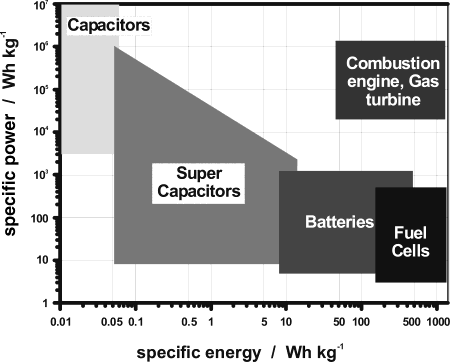
\includegraphics[width=0.48\textwidth]{specific-power-energy}
	\caption{Ragone plot --- Comparison energy density (specific energy) and power density (specific power) of most common storage domains \cite{winter2004batteries}.}
	\label{Fig:power-vs-energy-1}
\end{figure}

\begin{figure}
	\centering
	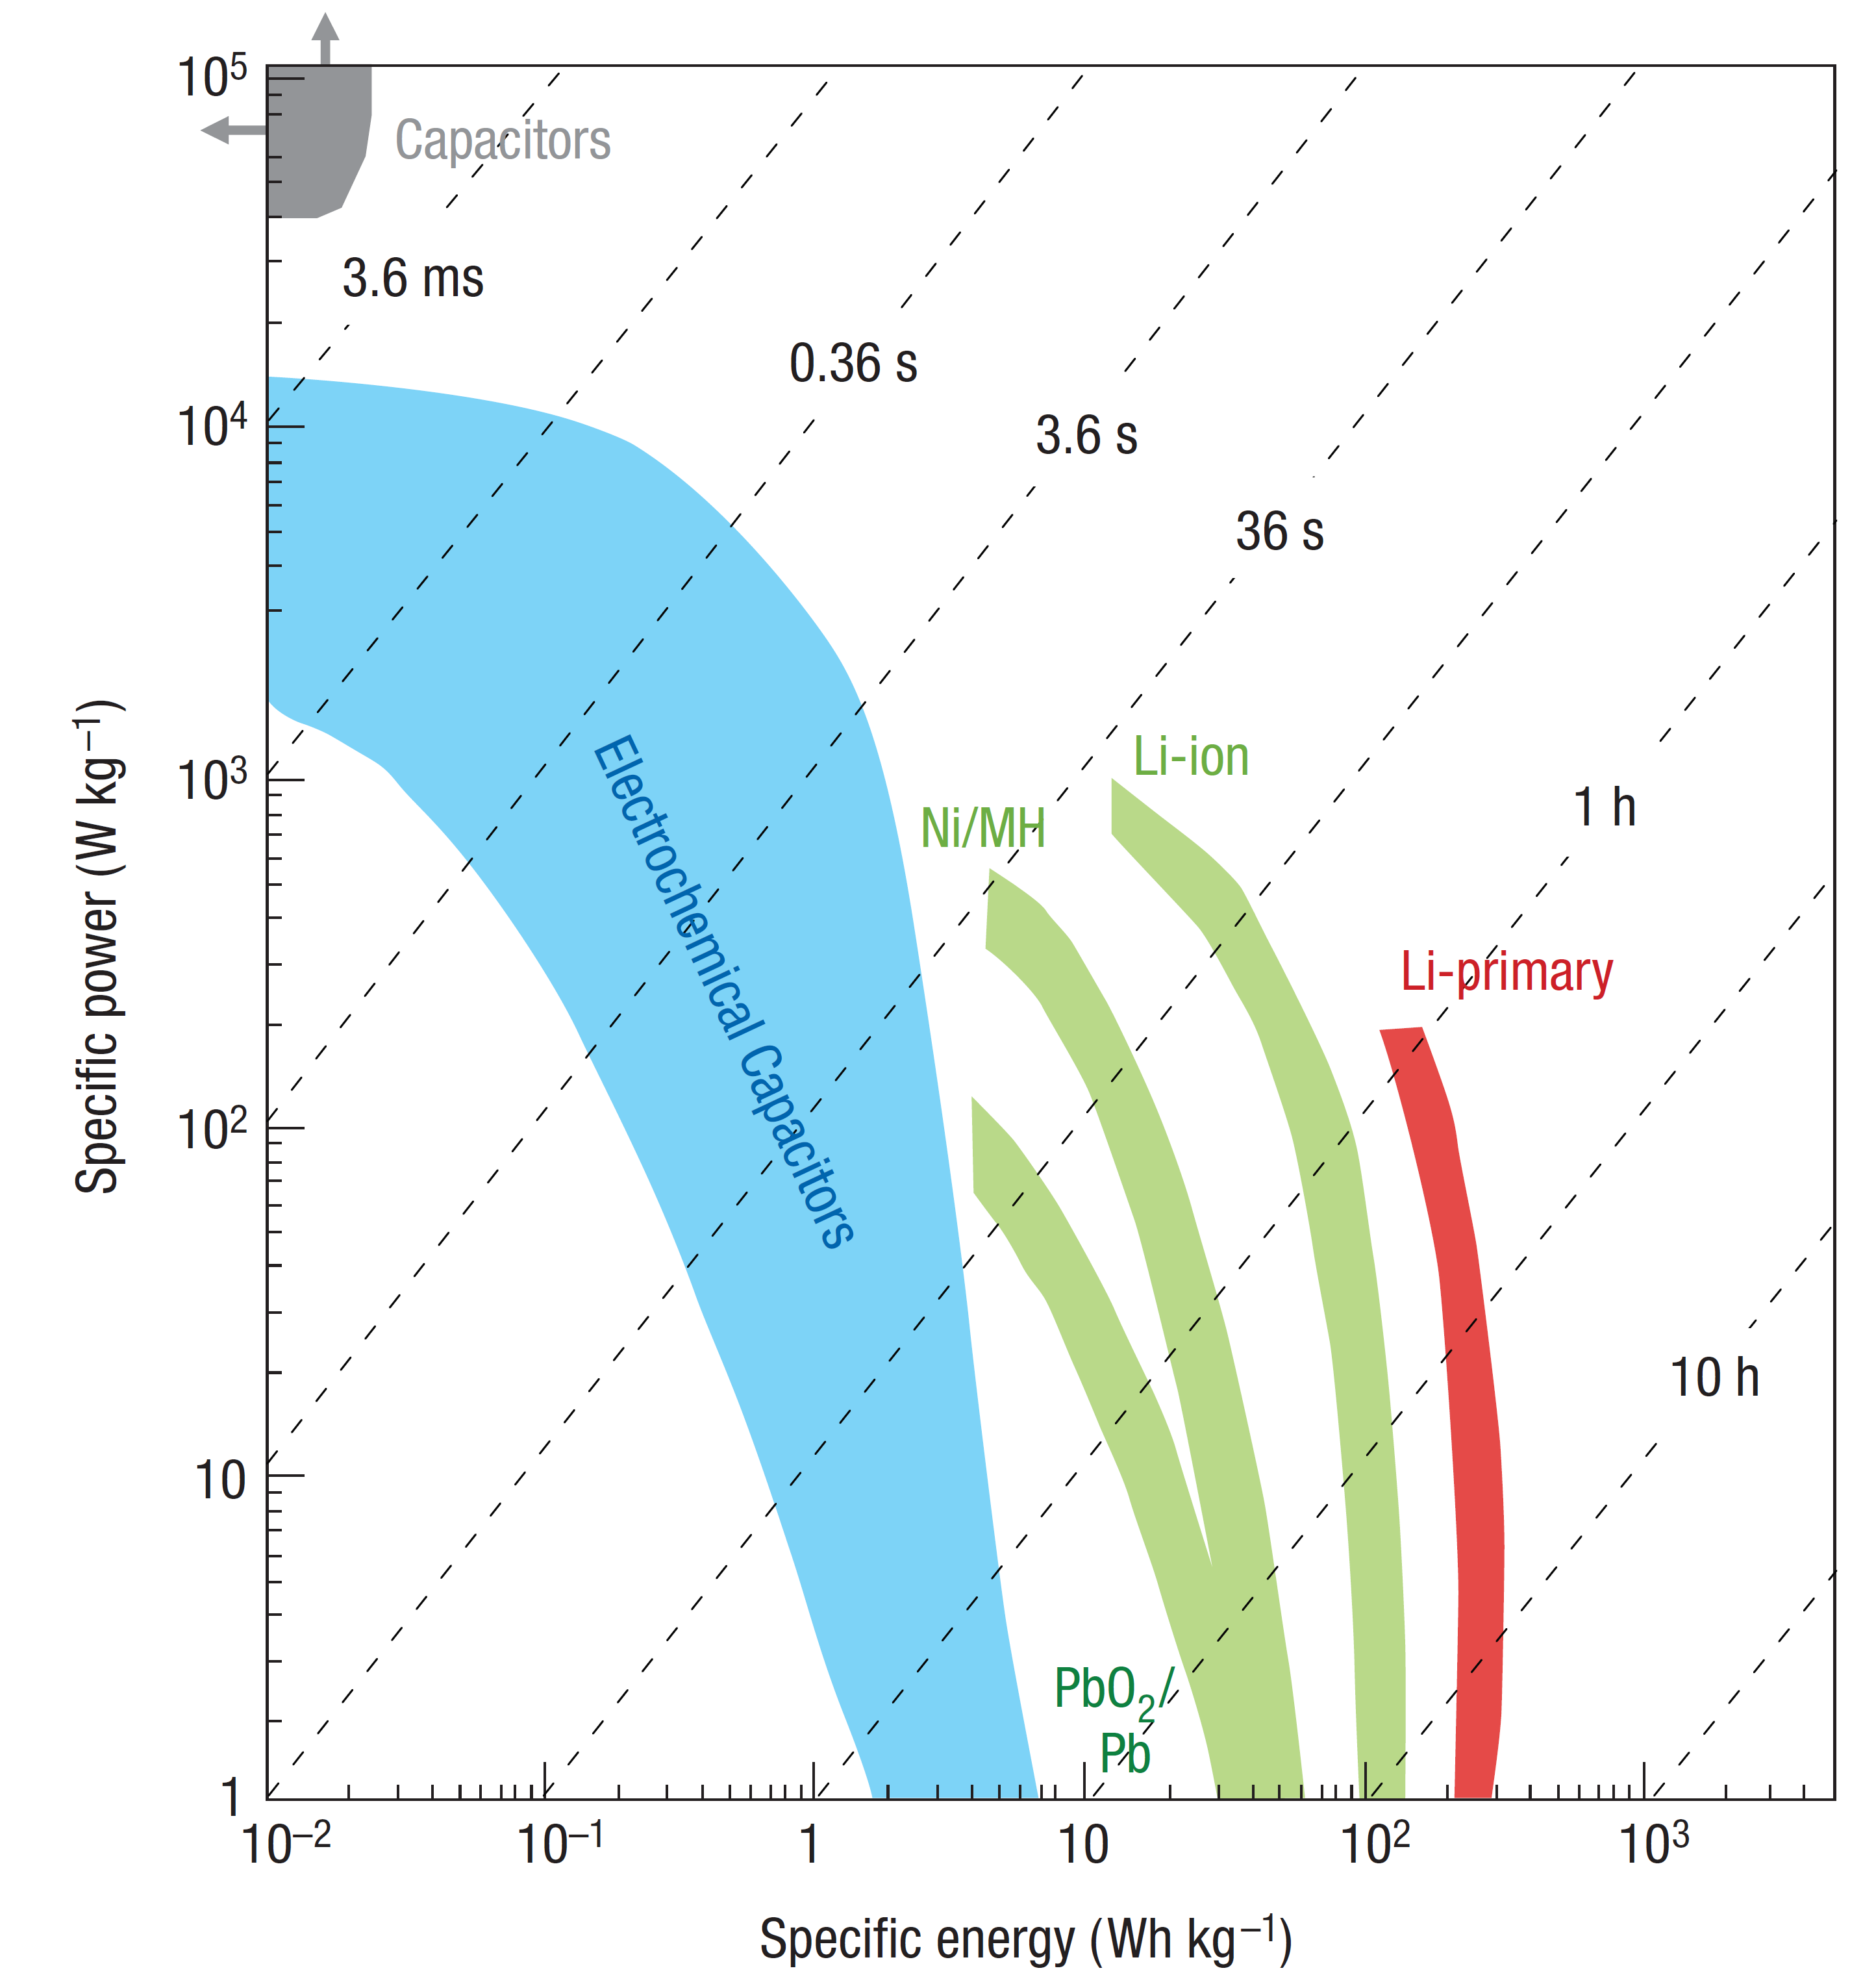
\includegraphics[width=0.48\textwidth]{power-vs-energy-density}
	\caption{Ragone plot --- Comparison energy density (specific energy) and power density (specific power) of various electric power storages \cite{simon2008materials}.}
	\label{Fig:power-vs-energy-2}
\end{figure}


\bibliographystyle{IEEEtran}
\bibliography{refs}

\end{document}